\section{Introduction}\label{introduction}

\begin{frame}{Women Contribute Online Less Than Men}

\begin{itemize}[<+->]
\tightlist
\item
  Only 13\% women contributors on Wikipedia
\item
  Wikipedia entries about women are less likely to be complete
\item
  Only 5\% women contributors on StackOverflow
\item
  Less than 5\% women taking part in programming competitions (despite
  30\% in CS schools)
\end{itemize}

\end{frame}

\begin{frame}{Implications for individuals, firms \& society}

\textbf{Profit loss} of online companies (e.g., Airbnb)

\begin{itemize}
\tightlist
\item
  Narrow participation
\item
  Less diversity \& creativity for innovation
\end{itemize}

\pause

\textbf{Labor market discrimination}

\begin{itemize}
\tightlist
\item
  Signaling skills
\item
  Learning
\end{itemize}

\pause

\textbf{Cultural} discrimination

\begin{itemize}
\tightlist
\item
  Platform content may reflect biased views
\end{itemize}

\end{frame}

\begin{frame}{A theory of gender imbalance}

Many factors to consider (see Lam et. al 2011)

We conjecture:

\begin{itemize}
\tightlist
\item
  \textbf{Gamification} \& Incentives (e.g., competition, points,
  rankings)
\item
  Gender differences in \textbf{preferences} (e.g., risk aversion,
  competitive inclination)
\end{itemize}

\pause

\textbf{Mechanisms} under investigation

\begin{enumerate}
\def\labelenumi{\arabic{enumi}.}
\tightlist
\item
  Perceived gender composition in a competitive environment.
\item
  \color{gray}{Collaboration incentives under gender imbalance [next study]}
\end{enumerate}

\end{frame}

\section{The role of the perceived gender
imbalance}\label{the-role-of-the-perceived-gender-imbalance}

\begin{frame}{Bayesian updating}

\begin{figure}
\centering
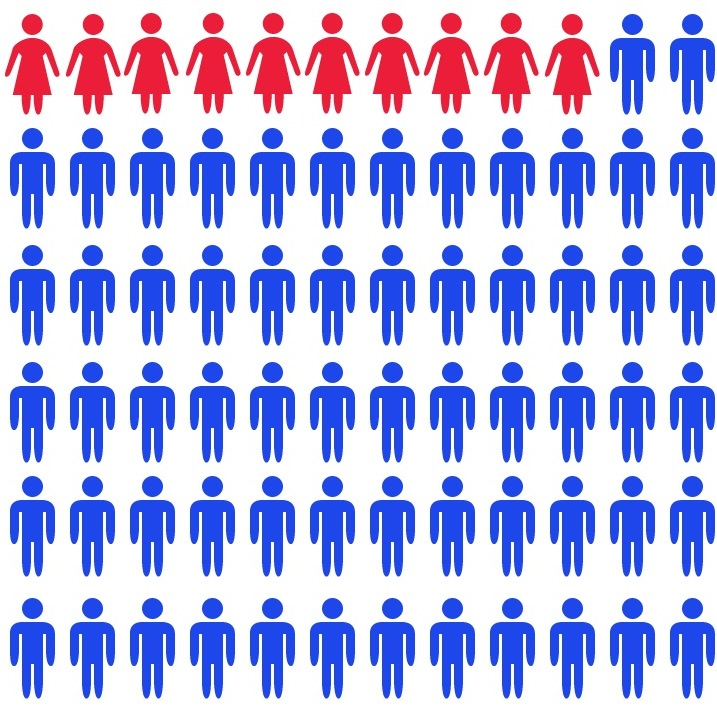
\includegraphics{female_fuel_for_the_digital_economy.jpg}
\caption{What are the odds of winning for gender XY?}
\end{figure}

\end{frame}

\begin{frame}{Role model}

\begin{figure}
\centering
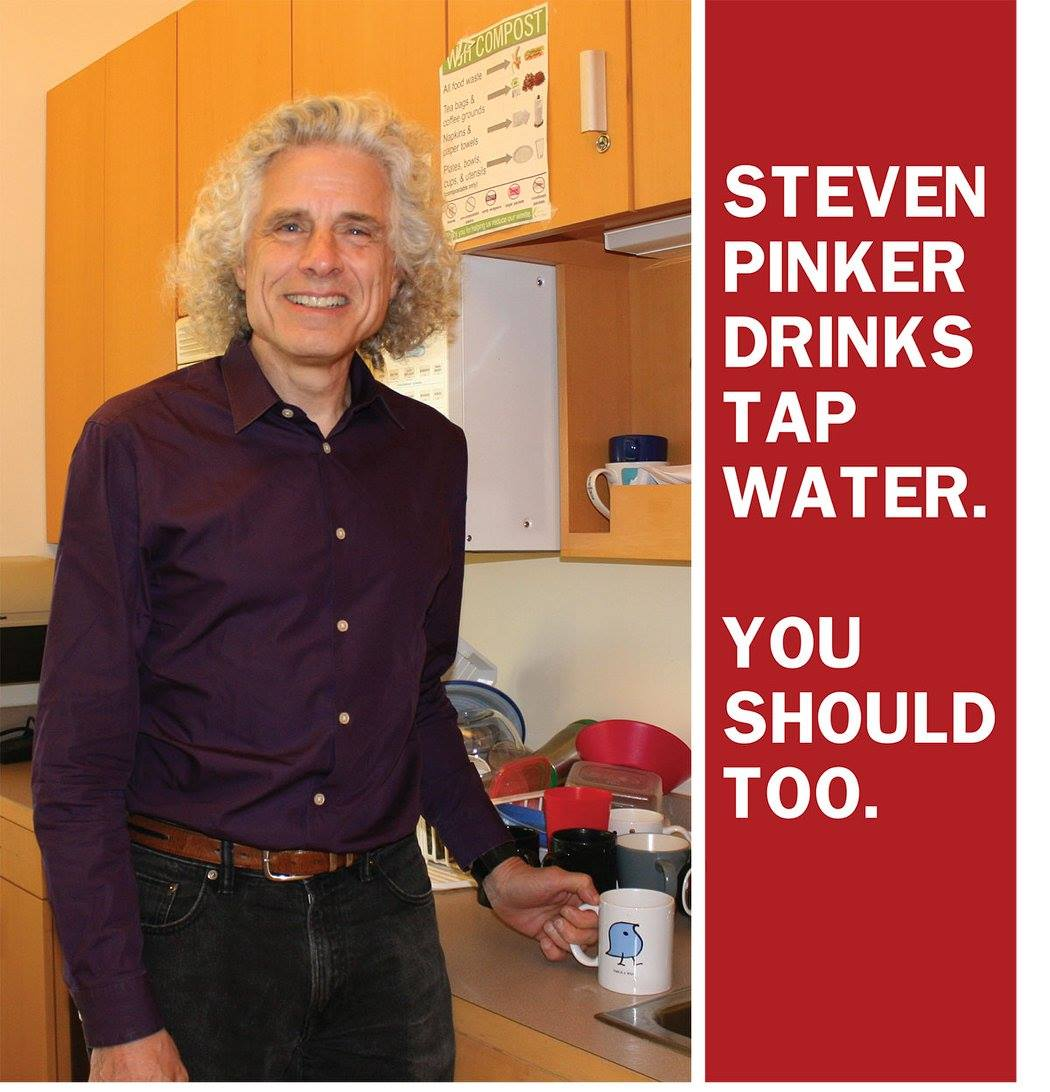
\includegraphics[width=0.5\textwidth]{tap_water_pinker.jpg}
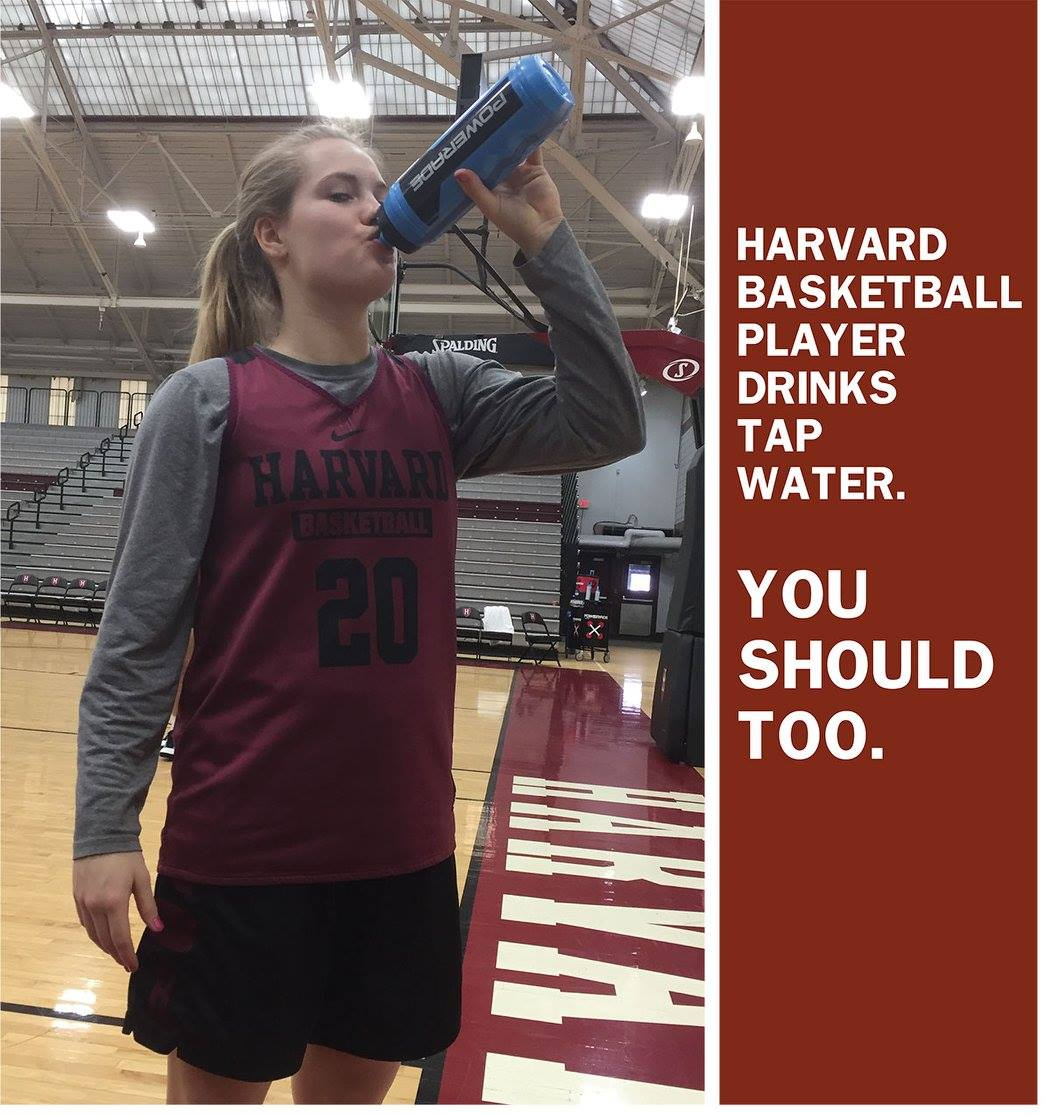
\includegraphics[width=0.5\textwidth]{tap_water_basket.jpg}
\caption{do I want to be successful in this?}
\end{figure}

\end{frame}

\begin{frame}

\begin{figure}
\centering
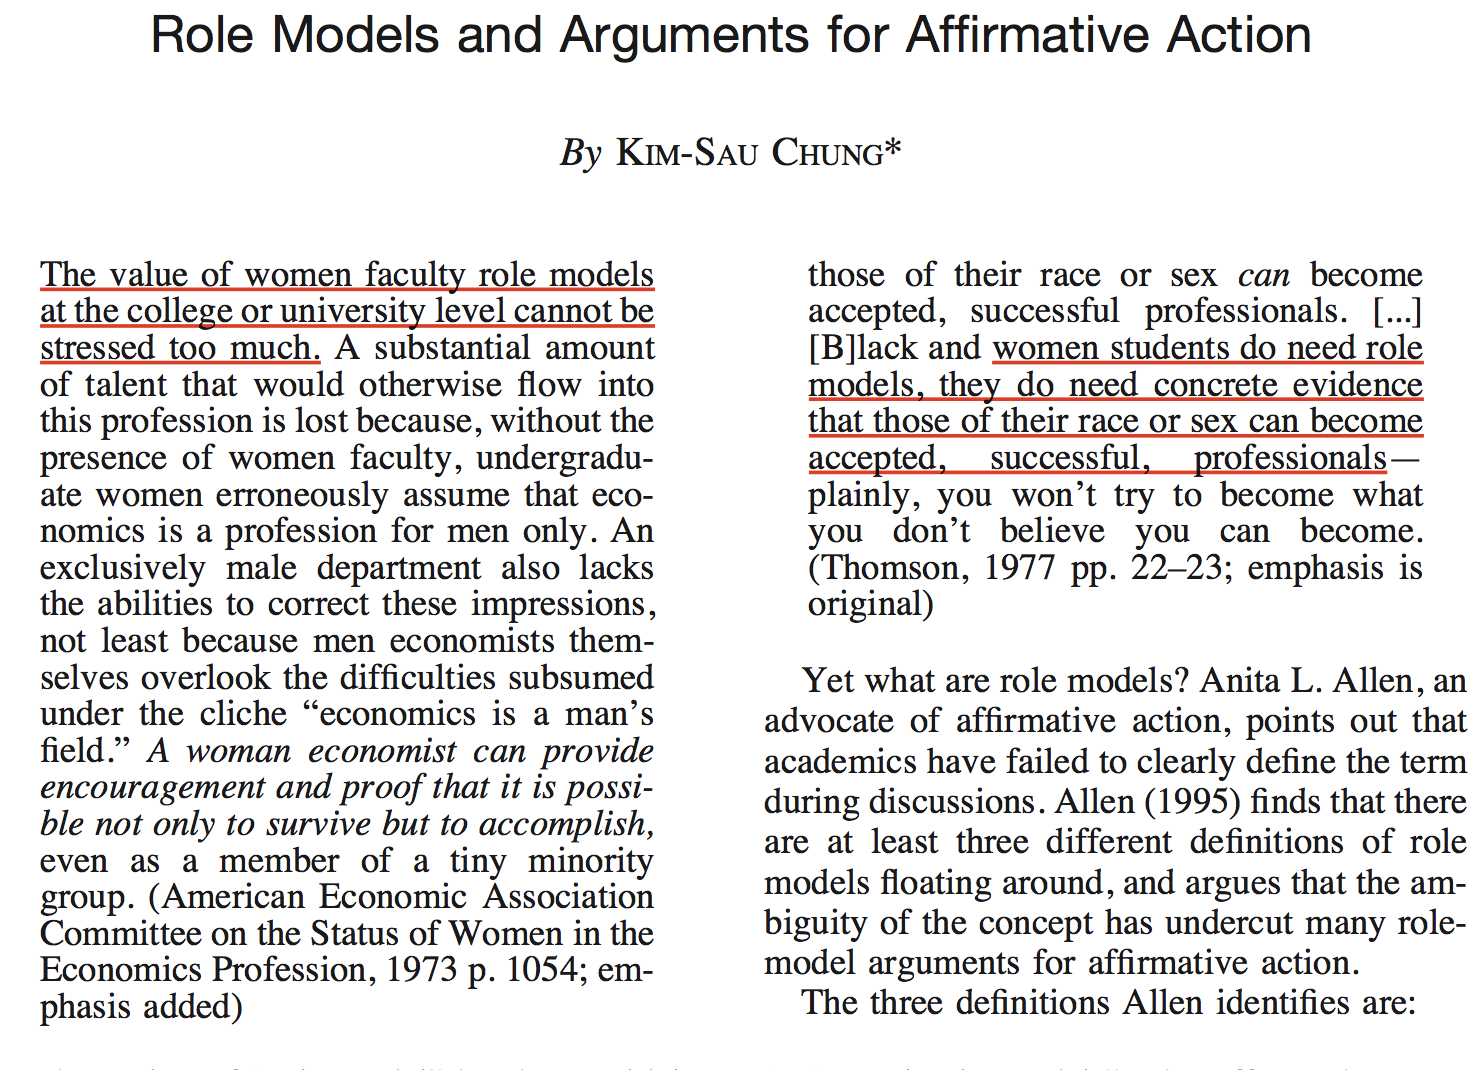
\includegraphics{aer-citation.png}
\caption{American Economic Review, 2000}
\end{figure}

\end{frame}

\section{Context and Data}\label{context-and-data}

\begin{frame}{Herox.com}

The sex ratio is:

\begin{itemize}
\tightlist
\item
  \textbf{2 men registrants} for a woman (33 percent women)
\item
  \textbf{2.8 men contributors} for a women (26 percent women)
\end{itemize}

\end{frame}

\begin{frame}

\begin{figure}
\centering
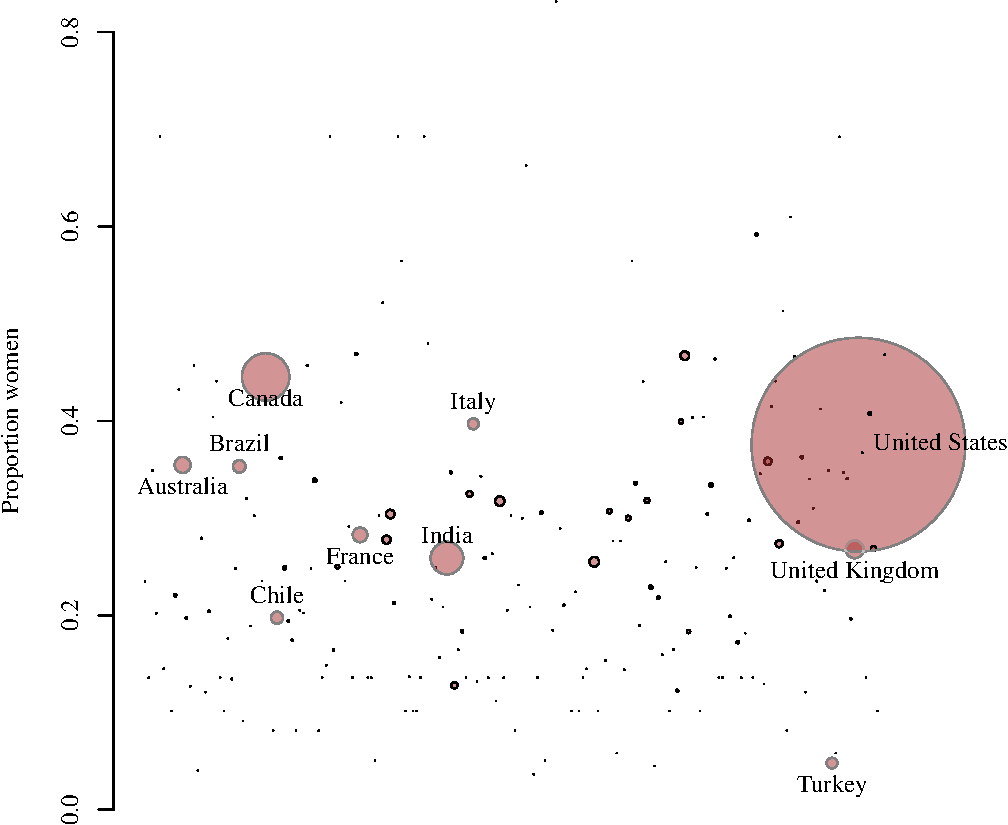
\includegraphics{deck_files/figure-beamer/bayes-1.pdf}
\caption{Proportion of women members by country}
\end{figure}

\end{frame}

\begin{frame}

\begin{figure}
\centering
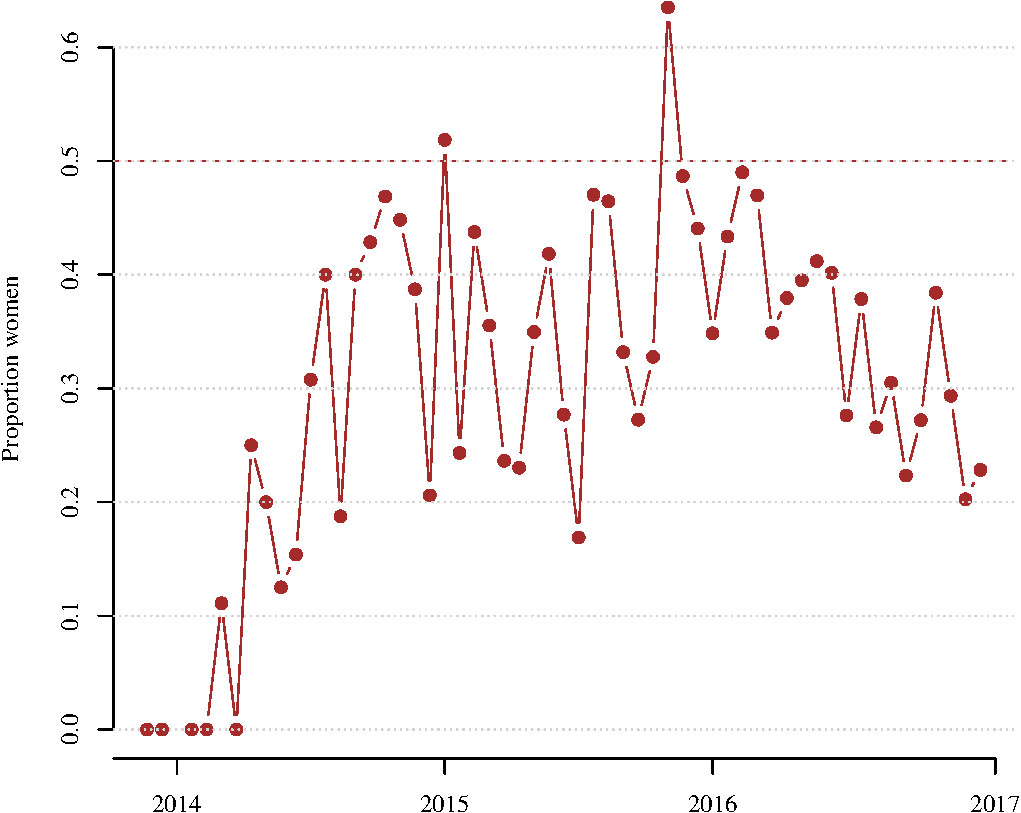
\includegraphics{deck_files/figure-beamer/overtime-1.pdf}
\caption{Proportion of women members over time}
\end{figure}

\end{frame}

\begin{frame}{How to influence the perceived gender composition?}

Solicitation via email featuring 2-3 member profiles.

\begin{itemize}
\item
  experience + bio + profile picture
\item
  ADD regression controls for past experience on platform
\end{itemize}

\end{frame}

\begin{frame}{Example}

\begin{figure}
\centering
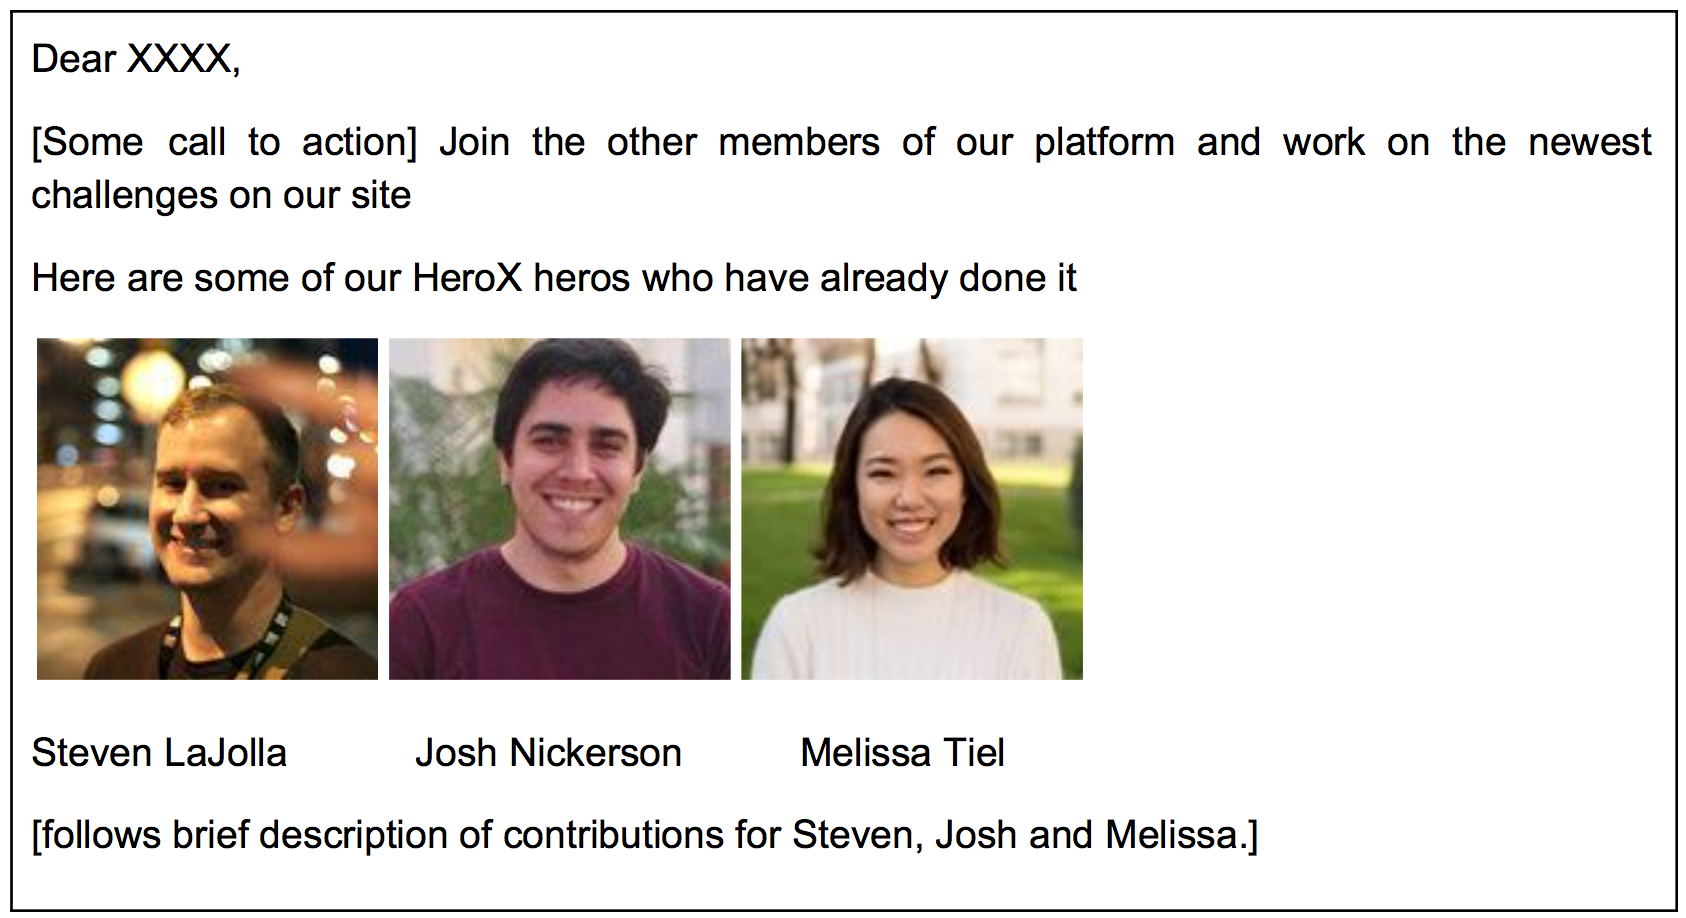
\includegraphics{solicit_gender_compo.png}
\caption{Solicitation email}
\end{figure}

\end{frame}

\begin{frame}{Treatment}

\begin{itemize}
\tightlist
\item
  Vary gender composition
\item
  Vary ``success'' composition
\end{itemize}

\begin{table}[ht]
\centering
\begin{tabular}{rll}
  \hline
 & Var1 & Var2 \\ 
  \hline
1 & 1 man role model & 3 women \\ 
  2 & 1 woman role model & 3 women \\ 
  3 & 1 man role model & 1 man 2 women \\ 
  4 & 1 woman role model & 1 man 2 women \\ 
  5 & 1 man role model & 2 men 1 woman \\ 
  6 & 1 woman role model & 2 men 1 woman \\ 
  7 & 1 man role model & 3 men \\ 
  8 & 1 woman role model & 3 men \\ 
   \hline
\end{tabular}
\caption{Treatment combinations} 
\end{table}

\end{frame}

\begin{frame}{Validation of profiles}

Goal: comparable profiles

Use demographics + AMT ratings of 20-30 profiles

\begin{itemize}
\tightlist
\item
  Physical attractiveness (based on user profile picture)
\item
  Role model (bio description + picture)
\item
  Skills
\end{itemize}

\end{frame}

\begin{frame}{Timing of the experiment}

\begin{enumerate}
\def\labelenumi{\arabic{enumi}.}
\tightlist
\item
  Preliminary survey (calibrate perceived gender composition)
\item
  Solicitation (email sent 1-2 times)
\item
  Ex-post survey (detect possible changes on perceived gender
  composition)
\end{enumerate}

\begin{itemize}
\tightlist
\item
  Outcome variables: participation, effort, team formation, etc.
\end{itemize}

\end{frame}

\begin{frame}{Next steps}

\begin{itemize}
\tightlist
\item
  Experiment on teaming on the platform
\item
  Wikipedia collaboration
\end{itemize}

\end{frame}

\begin{frame}{Example teaming}

\begin{figure}
\centering
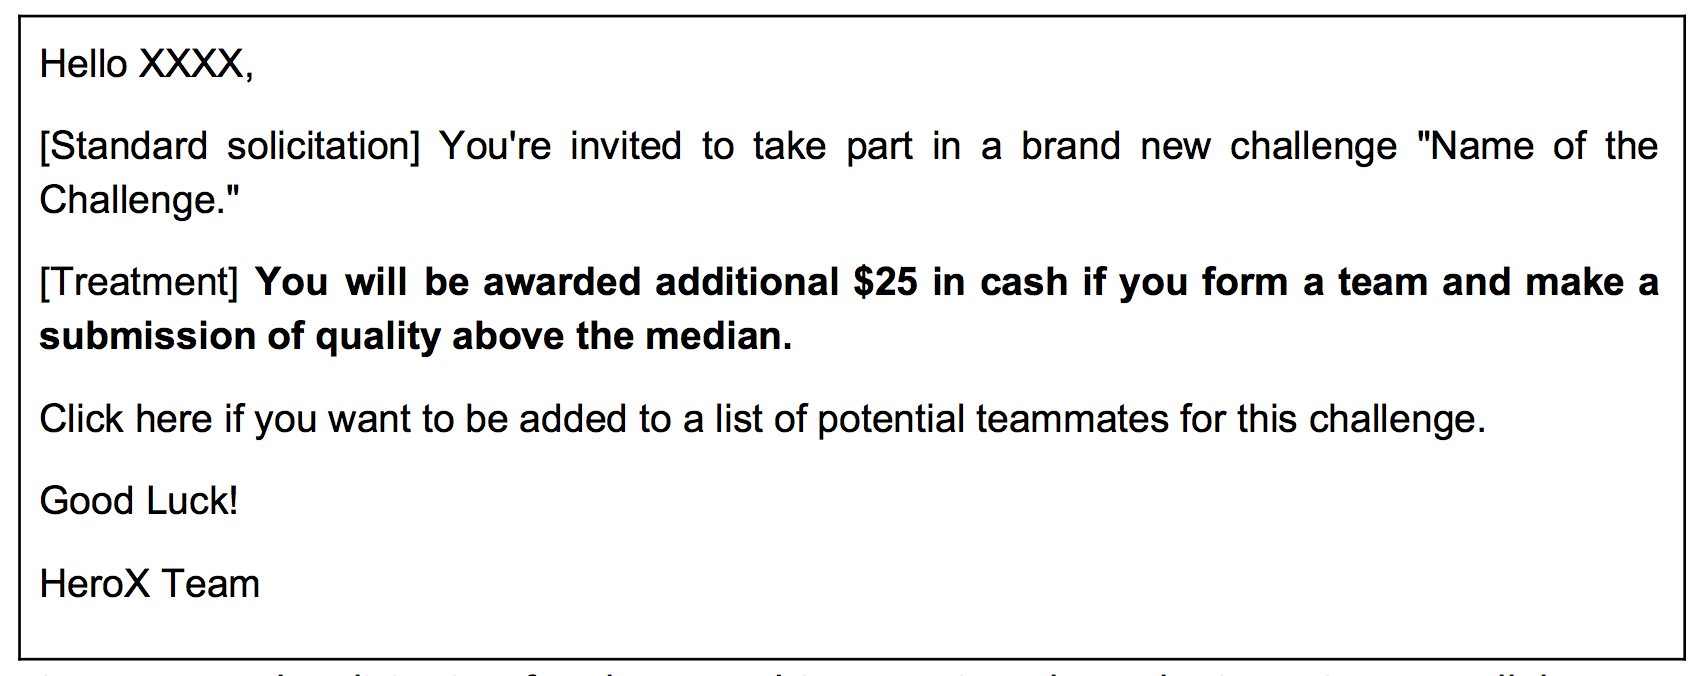
\includegraphics{solicit_teaming.png}
\caption{Teaming experiment}
\end{figure}

\end{frame}

\begin{frame}{Treatments}

\begin{enumerate}
\def\labelenumi{\arabic{enumi}.}
\tightlist
\item
  Male-female rich environment (how many teams?)
\item
  Splitting the pie rules (how many teams?)
\item
  Confidence
\end{enumerate}

\end{frame}

\begin{frame}{TODOS}

\begin{itemize}
\item
  Ask HeroX about winners
\item
  Ask Facebook ads
\item
  Tokenism
\end{itemize}

Interesting paper:

\url{https://papers.ssrn.com/sol3/papers.cfm?abstract_id=2804265}

\end{frame}
